%%%%%%%%%%%%%%%%%%%%%%%%%%%%%%%%%%%%%%%%%
% Simple Sectioned Essay Template
% LaTeX Template
%
% This template has been downloaded from:
% http://www.latextemplates.com
%
% Note:
% The \lipsum[#] commands throughout this template generate dummy text
% to fill the template out. These commands should all be removed when 
% writing essay content.
%%%%%%%%%%%%%%%%%%%%%%%%%%%%%%%%%%%%%%%%%

%----------------------------------------------------------------------------------------
%	PACKAGES AND OTHER DOCUMENT CONFIGURATIONS
%----------------------------------------------------------------------------------------

\documentclass[12pt]{book} % Default font size is 12pt, it can be changed here
		\textheight = 28cm
		\textwidth = 19cm
		\topmargin = -1cm
		\oddsidemargin = -1cm
		\parindent = 5mm

\usepackage{geometry} % Required to change the page size to A4
\geometry{a4paper} % Set the page size to be A4 as opposed to the default US Letter

\usepackage{graphicx} % Required for including pictures

\usepackage{float} % Allows putting an [H] in \begin{figure} to specify the exact location of the figure
\usepackage{wrapfig} % Allows in-line images such as the example fish picture

%\usepackage{lipsum} % Used for inserting dummy 'Lorem ipsum' text into the template

\linespread{1.1} % Line spacing

%\setlength\parindent{0pt} % Uncomment to remove all indentation from paragraphs
\usepackage[utf8]{inputenc}
\usepackage[spanish]{babel}
\usepackage[T1]{fontenc}
\usepackage{fancyhdr}
\usepackage{multicol}

% Configurar los encabezados, pies de pagina y paginas de capitulo
% Encabezados
\lhead[\thepage]{CAPÍTULO \thechapter. \rightmark}
\chead[]{}
\rhead[CAPÍTULO \thechapter. \leftmark]{\thepage}

\renewcommand{\headrulewidth}{0.5pt}

% Pie de pagina

\lfoot[]{\today}
\cfoot[]{}
\rfoot[J.Carlos Ávila]{}
\renewcommand{\footrulewidth}{0pt}

\usepackage{savesym}
\usepackage{amsmath}
\savesymbol{iint}
\usepackage{txfonts}
\restoresymbol{TXF}{iint}


\usepackage[x11names,table]{xcolor}
\usepackage{pstricks}
\usepackage[colorinlistoftodos, textwidth=2cm, shadow]{todonotes}
%\usepackage{hyperref}



\usepackage[colorlinks]{hyperref}
\usepackage[nogroupskip,nopostdot]{glossaries}
\setglossarystyle{altlist}
\makenoidxglossaries




%\usepackage[toc,style=altlistgroup,hyperfirst=false]{glossaries}


\hypersetup{
    colorlinks=true,
    linkcolor=rosa1,
    filecolor=magenta,      
    urlcolor=cyan,
}

\urlstyle{same}

\graphicspath{{./images/}} % Specifies the directory where pictures are stored

\definecolor{miorange}{rgb}{0.11, 0.43, 0.21}
\definecolor{rosa1}{RGB}{236, 46, 80}

%%%%%%%%%%%%%%%%%%%%%%%%%%%%%%%%%%%%%%%%%%%%%%%%%%%%%%%%%%%%%%%%%%%%%%%%%%%%%%%%%%%%%%%%%%%%%%%%%%%%%%%%%%%
%----------------------------------------------------------------------------------------
%	begin {Glosario}
%----------------------------------------------------------------------------------------

\newglossaryentry{SO}{name={SO},description={Es el sistema o conjunto de aplicaciones que permiten que una computadora lleven a cabo sus funciones.}}
\newglossaryentry{Linux}{name={Linux},description={GNU/Linux Sistema Operativo creado y distribuido por miles de 
													personas alrededor del mundo}}
													
\newglossaryentry{Windows}{name={Windows},description={Sistema Operativo creado y distribuido por Microsoft.}}

\newglossaryentry{Mac}{name={Mac},description={Sistema Operativo creado y distribuido por Apple}}

%%%%%%%%%%%%%%%%%%%%%%%%%%%%%%%%%%%%%%%%%%%%%%%%  %%%%%%%%%%%%%%%%%%%%%%%%%%%%%%%%%%%%%%%%%%%%%%%%%%%%%%%%%
\newglossaryentry{}{name={},description={}}
%%%%%%%%%%%%%%%%%%%%%%%%%%%%%%%%%%%%%%%%%%%%%%%%  %%%%%%%%%%%%%%%%%%%%%%%%%%%%%%%%%%%%%%%%%%%%%%%%%%%%%%%%%

%----------------------------------------------------------------------------------------
%	End {Glosario}
%----------------------------------------------------------------------------------------


\pagestyle{fancy}

\begin{document}

\lhead[\thepage]{CAPÍTULO \thechapter. \rightmark}
\rhead[CAPÍTULO \thechapter. \leftmark]{\thepage}


%----------------------------------------------------------------------------------------
%	TITLE PAGE
%----------------------------------------------------------------------------------------

\begin{titlepage}

\newcommand{\HRule}{\rule{\linewidth}{0.5mm}} % Defines a new command for the horizontal lines, change thickness here

\center % Center everything on the page
 
%----------------------------------------------------------------------------------------
%	HEADING SECTIONS
%----------------------------------------------------------------------------------------

\textsc{\LARGE Instituto Tecnológico de San Juan del Río}\\[1.5cm] % Name of your university/college
\textsc{\Large Centro de Investigación en ciencia Aplicada y Tecnología Avanzada}\\[0.5cm] % Major heading such as course name
%\textsc{\large Minor Heading}\\[0.5cm] % Minor heading such as course title

%----------------------------------------------------------------------------------------
%	TITLE SECTION
%----------------------------------------------------------------------------------------

\HRule \\[0.4cm]
{ \huge \bfseries Amplificación interactiva de contenido por medio de la detección de la dirección de la mirada.}\\[0.4cm] % Title of your document
\HRule \\[1.5cm]
 
%----------------------------------------------------------------------------------------
%	AUTHOR SECTION
%----------------------------------------------------------------------------------------

\begin{minipage}{0.4\textwidth}
\begin{flushleft} \large
\emph{Autor:}\\
J. Carlos \textsc{\'Avila Resendiz} % Your name
\end{flushleft}
\end{minipage}
~
\begin{minipage}{0.4\textwidth}
\begin{flushright} \large
\emph{Supervisor:} \\
Dr. Joaquin  \textsc{Salas Rodriguez} % Supervisor's Name
\end{flushright}
\end{minipage}\\[4cm]

% If you don't want a supervisor, uncomment the two lines below and remove the section above
%\Large \emph{Author:}\\
%John \textsc{Smith}\\[3cm] % Your name


%----------------------------------------------------------------------------------------
%	DATE SECTION
%----------------------------------------------------------------------------------------

{\large \today}\\[1cm] % Date, change the \today to a set date if you want to be precise

%----------------------------------------------------------------------------------------
%	LOGO SECTION
%----------------------------------------------------------------------------------------


\includegraphics{./imagenes/itsjr_s.jpg}\\ % Include a department/university logo - this will require the graphicx package

 
%----------------------------------------------------------------------------------------

\vfill % Fill the rest of the page with whitespace
\newpage
$\ $
\thispagestyle{empty}
\end{titlepage}

%----------------------------------------------------------------------------------------
%	TABLE OF CONTENTS
%----------------------------------------------------------------------------------------j
\setcounter{tocdepth}{3}   %control deptness index
%\setcounter{lofdepth}{2}  % control table of figures depth 
\pagenumbering{roman} 
\tableofcontents % Include a table of contents

\newpage % Begins the essay on a new page instead of on the same page as the table of contents
\thispagestyle{empty} 
%\appendix
%----------------------------------------------------------------------------------------
%	INTRODUCTION
%----------------------------------------------------------------------------------------
\pagenumbering{arabic}	
%\setcounter{page}{1}
	
			 
\newpage		 
\pagestyle{fancy}


\chapter{GENERALIDADES}
\thispagestyle{empty}
\markboth{GENERALIDADES}{GENERALIDADES}

\begin{minipage}{0.5\textwidth}
	\begin{flushleft} \large
	%\emph{•} \\
	\scriptsize	\textsl{\large “El auténtico genio consiste en la capacidad para evaluar información incierta, 
								aleatoria y contradictoria.”}\\
	\scriptsize \textbf{Winston Churchill, estadista.}
	\end{flushleft}
\end{minipage}\\[4cm]			

\newpage
\section{Objetivos}
	\subsection{Objetivo general}
	
		Desarrollar una aplicación de amplificación interactiva para computadoras con sistema operativo Windows, 
		que asista a personas con bajas capacidades visuales, por medio del seguimiento y estimación de la dirección 
		de la mirada sobre la pantalla de la computadora y en base a ello amplificar la zona de la pantalla en la 
		que enfoca la vista.
	
	\subsection{Objetivos específicos}
		\begin{itemize}
			\item Detección precisa y confiable del movimiento del globo ocular, con la ayuda de software de 
			procesamiento de imágenes digitales.
			\item Hacer uso de las API’s del sistema operativo que proveen las herramientas que magnifican la zona de
			la pantalla seleccionada.
			\item Integrar los dos componentes anteriores y de esa forma obtener un magnificador con interacción visual.
			\item Una vez se cuente con un prototipo, realizar pruebas de campo.
		\end{itemize}
		

\newpage
\section{Justificación}
	Pese al avance desmesurado de la tecnología en los últimos años en donde las capacidades de los dispositivos se
	duplica cada cierto tiempo, respondiendo de forma bastante precisa la emblemática ley de 
	\href{https://en.wikipedia.org/wiki/Moore's_law}{Moore} hay aun a día de hoy
	ciertas cuestiones que no han sido abordadas, quizá en gran parte debido al amplio panorama de problemas que se
	pueden afrontar con soluciones tecnológicas y de alguna forma ayudar a solventar o/y hacer más fácil las mismas.
	
	Aun si los programas de asistencia a personas con capacidades diferentes están a día de hoy cobrando mayor 			  	
	relevancia en prácticamente todos los aspectos sociales, pues en la actualidad las posibilidades de llevar una vida
	productiva y sin las limitaciones de antaño, son ya una realidad, entre las herramientas que se proporcionan a este
	sector de la población están las llamadas tecnologías de asistencia o accesibilidad en entornos informáticos, mismas
	que van desde iconos monocromáticos de un mayor tamaño, hasta lectores de pantalla y lupas, siendo estas últimas el
	principal componente proporcionado por las herramientas de accesibilidad de los Sistemas Operativos \gls{SO} actuales,
	siendo común en los tres mas importantes \gls{Linux}, \gls{Windows}, \gls{Mac}.
	
	Siendo de los tres el segundo, Windows, en el cual se enfocaran los esfuerzos de hacer converger las herramientas de
	accesibilidad ya mencionadas y las tecnologías de visión por computadora CV, para ofrecer a los discapacitados 
	visuales una forma de hacer uso de la tecnología, mismos que según datos de la OMS de 2002, eran mas de 161 millones
	de personas, en especifico de computadoras, sin que su limitante visual les impida el poder interactuar con el 
	equipo.
	
	Específicamente el segmento de la población con discapacidad visual en el que se enfoca el desarrollo de este
	proyecto es el de personas que cuentan con cierto grado de visión, o lo que se conoce como resto visual, pues,
	siempre que exista un resto visual por mínimo que sea se debe potenciar su uso para alcanzar el máximo desarrollo
	posible

\newpage 
\section{Caracterización de la empresa}
	\subsection{Datos generales de la empresa}
	\begin{description}
		\item[Nombre de la organización:] Centro de Investigación en Ciencia Aplicada y Tecnología Avanzada del
			 Instituto Politécnico Nacional \texttt{CICATA}
			 
		\item[Dirección:] Querétaro, Cerro Blanco No.141 Col. Colinas del Cimatario, C.P. 76090, Querétaro, Querétaro
			 México.
			 \begin{center}
			 	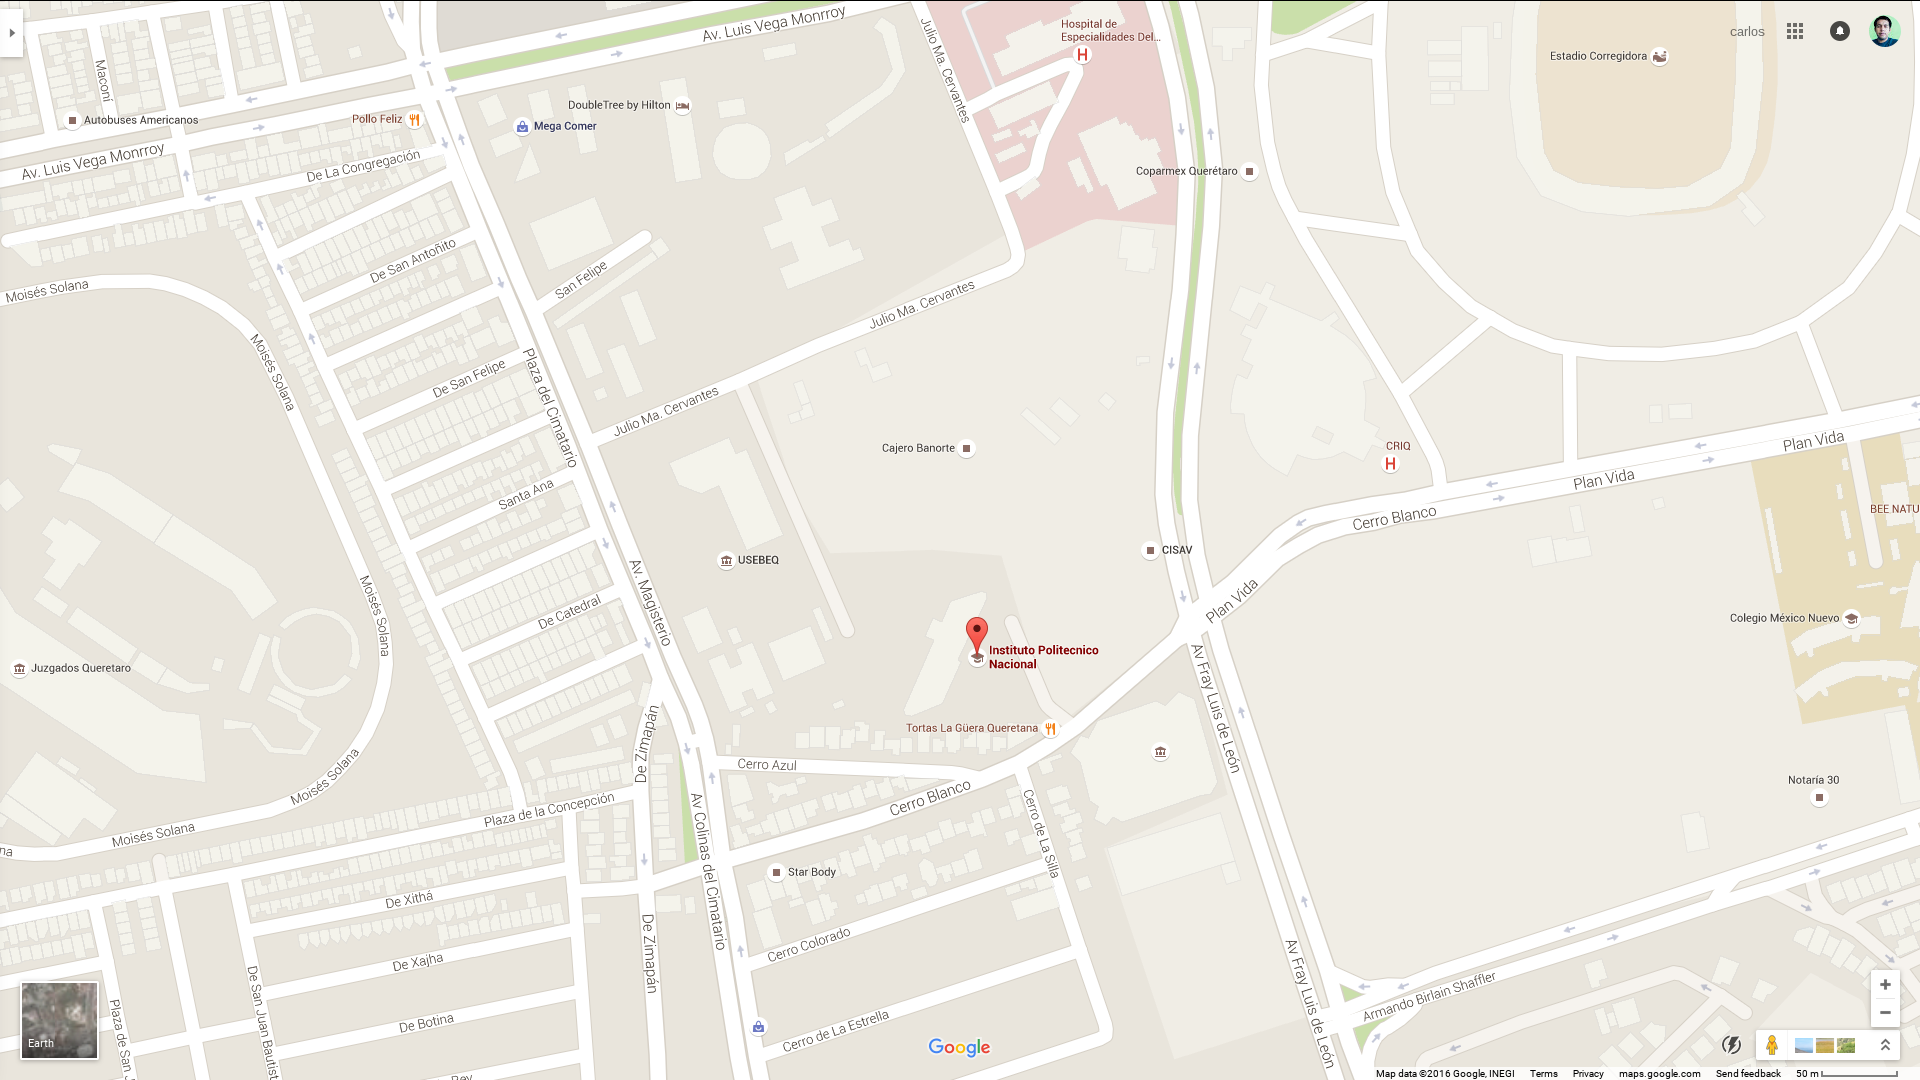
\includegraphics[width=0.9\textwidth]{./imagenes/cicata}
			 \end{center}
		\item[Teléfonos:] 1 (442) 2290804 o 01 (55) 5729 6000 Ext. 81002
		\item[E-Mail:] cicata@ipn.mx 
		\item[Fax:] 5395 4147
	\end{description}
		\subsubsection{Misión}
			Somos un centro de investigación creado por el IPN para fortalecer su impacto a nivel nacional, que atiende
			necesidades de formación de recursos humanos y de desarrollo tecnológico de la región, a través de proyectos
			de investigación que contribuyen al desarrollo social y a la competitividad de los sectores productivo y de
			servicios, con el respaldo de las capacidades del Instituto, con un enfoque multidisciplinario, innovador y
			de excelencia, en un marco de sustentabilidad.
		
		\subsubsection{Visión}
			En el 2025, el CICATA-Querétaro se ve como un centro de vanguardia en la investigación y formación de 
			recursos humanos; referente a nivel latinoamericano; con reconocimiento internacional por sus contribuciones
			de alto impacto y como una de las primeras opciones para alumnos e investigadores, por ser un centro
			innovador, competitivo, líder y emprendedor.
		
		\subsubsection{Valores}
			Hemos identificado un conjunto de valores que nos representan y que permiten cumplir nuestra misión y lograr
			la visión forjada:\\
			\begin{multicols}{2}
				\begin{itemize}
					\item Calidad
					\item Integridad
					\item Compromiso
					\item Asertividad
					\item Trabajo en equipo
					\item Aprendizaje continuo
				\end{itemize}
			\end{multicols}
		
		\subsubsection{Objetivo}
			Servir de enlace entre la comunidad científica y los sectores productivos de bienes y servicios, atenderlos
			y ofrecerles soluciones a sus problemas de desarrollo. Para el cumplimiento de este objetivo, CICATA
			Querétaro desarrolla programas de investigación científica, tecnológica e innovación con un enfoque
			interdisciplinario, y asimismo atiende la formación de capital humano de alto nivel, contribuyendo
 			decisivamente al fortalecimiento de la calidad y la competitividad del aparato productivo mexicano.
 		
 		\subsubsection{Estructura Organizativa}
			 
	
	\subsection{Descripción del departamento o área de trabajo}

\newpage
\section{Problemas a resolver}

\newpage
\section{Alcances y limitaciones}
	\subsection{Alcances}
	\subsection{Limitaciones}




\chapter{FUNDAMENTACIÓN TEÓRICA}
\markboth{FUNDAMENTACIÓN TEÓRICA}{FUNDAMENTACIÓN TEÓRICA} 
\thispagestyle{empty}

\section{Ingeniería del software}

\section{Herramientas de desarrollo}
	
\section{Lenguajes de programación}
		\subsection{C++}
		\subsection{OpenCV}
		\subsection{IntraFace}

\section{Metodologías de desarrollo de software}
	\subsection{Metodología de desarrollo extremo \label{XP}}
		La programación extrema se basa en una serie de reglas y principios que se han ido gestando a lo largo de toda la historia de la 
		ingeniería del software. Usadas conjuntamente proporcionan una nueva metodología de desarrollo software que se puede englobar 
		dentro de las metodologías ligeras, que son aquéllas en la que se da prioridad a las tareas que dan resultados directos y que 
		reducen la burocracia que hay alrededor tanto como sea posible (pero no más).
		
		La programación extrema, dentro de las metodologías ágiles, se puede clasificar dentro de las evolutivas.
		
		Una de las características de \textsl{eXtreme Programming} es que muchos de, si no todos, sus ingredientes son de sobra conocidos
		dentro de la rama de la ingeniería del software desde hace tiempo, incluso desde sus comienzos. Los autores de han seleccionado 
		los que han considerados como los mejores y han profundizado en sus relaciones y en cómo se refuerzan unos a otros. El resultado 
		ha sido una metodología única y compacta. Por eso, a\'unque se pueda alegar que la programación extrema no se base en principios
		nada nuevos, se ha de aclarar que, en conjunto, es una nueva forma de ver el desarrollo de software. 
		
		\subsubsection{El proceso de desarrollo extremo}
			La programación extrema parte del caso habitual de una compañía que desarrolla software, generalmente software a medida, en la
			que hay diferentes roles: un equipo de gestión, un equipo de desarrolladores y los clientes. 
			La relación con el cliente es totalmente diferente a lo que se ha venido haciendo en las metodologías tradicionales que se basan
			fundamentalmente en una fase de captura de requisitos previa al desarrollo y una fase de validación posterior al mismo.
			 
		\subsubsection{Interacción con el cliente }
			En la programación extrema al cliente no sólo se le pide que apoye al equipo de desarrollo, en realidad podríamos decir que es 
			parte de él. Su importancia es capital a la hora de abordar las historias de los usuarios y las reuniones de planificación, como 
			veremos más adelante. Además, será tarea suya retroalimentar al equipo de desarrolladores después de cada iteración con los 
			problemas con los que se ha encontrado, mostrando sus prioridades, expresando sus sensaciones, etc.,
			
			Existirán métodos como pruebas de aceptación que ayudarán a que la labor del cliente sea lo más fructífera posible.
			
			En resumen, el cliente se encuentra mucho más cercano al proceso de desarrollo. Se elimina la fase inicial de captura de requisitos 
			y se permite que éstos se vayan definiendo de una forma ordenada durante el tiempo que dura el proyecto. El cliente puede cambiar 
			de opinión sobre la marcha y a cambio debe encontrarse siempre disponible para resolver dudas del equipo de desarrollo y para detallar 
			los requisitos especificados cuando sea necesario. 
			
			El proceso de captura de requisitos de XP gira entorno a una lista de características que el cliente desea que existan en el sistema 
			final. Cada una de estas características recibe el nombre de historias de usuarios y su definición consta de dos fases:
			
			\begin{description}
				\item[En la primera fase] el cliente describe con sus propias palabras las características y el responsable del equipo de 
					desarrollo le informa de la dificultad técnica de cada una de ellas y por lo tanto de su coste.
				\item[La segunda fase] consiste en coger las primeras historias que serán implementadas (primera iteración) y dividirlas 
					en las tareas necesarias para llevarlas a cabo.
			\end{description}
			
			Este proceso es una de las principales diferencias con las metodologías tradicionales. a\'unque las historias de usuarios guardan 
			cierta relación con otras técnicas como los casos de uso de UML, su proceso de creación es muy diferente. En lo que al cliente se 
			refiere no se le exige que especifique exactamente lo que quiere al principio con un documento de requisitos de usuario. La parte 
			que se mantiene con este documento es que es el cliente el que tiene que escribir lo que quiere, no se permite que alguien del 
			equipo de desarrolladores lo escriba por él.
			
		\subsubsection{Planificación del proyecto}
			 La planificación debe de seguir unas ciertas premisas. La primordial es que las entregas se hagan cuanto antes y que con cada 
			 iteración el cliente reciba una nueva versión. Cuanto más tiempo se tarde en introducir una parte esencial, menos tiempo habrá
			 para trabajar en ella posteriormente. Se aconsejan muchas entregas y muy frecuentes. De esta forma, un error en una parte esencial 
			 del sistema se encontrará pronto y, por tanto, se podrá arreglar antes.\\
			 
			 Sin embargo, los requisitos anteriores en cuanto a la planificación no deben suponer horas extra para el equipo de desarrollo.\\
			 
			 Pero lo mejor de todo es que a la hora de planificar uno se puede equivocar. Es más, todos sabemos que lo común es equivocarse 
			 y por ello la metodología ya tiene previsto mecanismos de revisión. Por tanto, es normal que cada 3 a 5 iteraciones se tengan 
			 que revisar las historias de los usuarios y renegociar nuevamente la planificación.\\
			 
		\subsubsection{Diseño, desarrollo y pruebas}
			El desarrollo es la pieza clave de todo el proceso de programación extrema. Todas las tareas tienen como objetivo que se desarrollo 
			a la máxima velocidad, sin interrupciones y siempre en la dirección correcta. 
			
			También se otorga una gran importancia al diseño y establece que éste debe ser revisado y mejorado de forma continua según se van 
			añadiendo funcionalidades al sistema.
			
			La clave del proceso de desarrollo de XP es la comunicación. La gran mayoría de los problemas en los proyectos de desarrollo son 
			provocados por falta de comunicación en el equipo, así que se pone un gran énfasis en facilitar que la información fluya lo más 
			eficientemente posible. 
			
			Como ya hemos visto con anterioridad, uno de los principios de la programación extrema es la simplicidad. El diseño debe ser lo 
			más simple posible, pero no más simple. El paradigma KISS ("Keep It Small and Simple" para unos o "Keep it Simple, Stupid" para otros) 
			se lleva hasta las últimas consecuencias. Por ejemplo, se hace énfasis en no añadir funcionalidad nunca antes de lo necesario, por las 
			sencillas razones de que probablemente ahora mismo no sea lo más prioritario o porque quizás nunca llegue a ser necesaria.
			
			
			Supongamos que ya hemos planificado y dividido en tareas, como se ha comentado en los párrafos anteriores. Lo lógico sería empezar 
			ya a codificar. Pues no. Nos encontramos con otro de los puntos clave de la programación extrema (y que sí es innovador en ella): 
			las pruebas unitarias se implementan a la vez hay que el código de producción. De hecho cada vez que se va a implementar una pequeña
			parte se escribe una prueba sencilla y luego el código suficiente para que la pase. Cuando la haya pasado se repite el proceso con 
			la siguiente parte.
			
			Esta forma de usar las pruebas unitarias ayuda a priorizar y comprobar la evolución del desarrollo y que ofrecen retroalimentación 
			inmediata.
			
			Ya no son imprescindibles dos equipos diferenciados que desarrollan y prueban cada uno por su cuenta. Ahora el ciclo se basa en 
			implementar una prueba unitaria, codificar la solución y pasar la prueba, con lo que se consigue un código simple y funcional de manera
			bastante rápida. Por eso es importante que las pruebas se pasen siempre al 100%. 
			 
			Las pruebas unitarias no se han de confundir con las pruebas de aceptación que han sido mencionadas con anterioridad. Éstas últimas son
			pruebas realizadas por el cliente o por el usuario final para constatar que el sistema hace realmente lo que él quiere.
			
			La programación extrema viene a perseguir lo que se ha venido a llamar integración continua. De esta forma, haciéndolo cada vez con 
			pequeños fragmentos de código, se evita la gran integración final. 
			
			En todo desarrollo de programación extrema debería existir, por tanto, una versión siempre integrada. La sincronización por parte de los
			desarrolladores con el repositorio central debe darse como mínimo una vez al día, de manera que los cambios siempre se realicen sobre 
			la última versión. De esta forma nos podemos asegurar de que las modificaciones que hacemos no se estén haciendo sobre una versión 
			obsoleta\\
			
			El proceso de desarrollo no lo va a hacer un desarrollador en solitario, sino siempre con otra persona, algo que se ha venido a llamar
			programación por parejas. Una pareja de desarrolladores debe compartir ordenador, teclado y ratón. El principal objetivo es realizar de 
			forma continua y sin parar el desarrollo una revisión de diseño y de código. Las parejas deben ir rotando de forma periódica para hacer 
			que el conocimiento del sistema se vaya difundiendo por el equipo (facilitándose que el código sea de todos), a la vez que se fomentan 
			el entrenamiento cruzado.
			
		\subsubsection{Resumen de XP}
			Todos los punto anteriormente detallados, bien los podemos definir y resumir en la siguiente lista, obviamente cada uno de ellos
			lleva consigo un gran significado de fondo, pero en general  y conociendo la metodología se puede uno basar en la siguiente lista 
			para cerciorarse de que se están cumpliendo los puntos que la metodología estipula que se deben llevar a cabo.
			
			\begin{enumerate}
				\item El juego de la planificación (the planning game).
				\item Pequeñas entregas (small releases).
				\item Metáfora (metaphor).
				\item Diseño simple (simple design).
				\item Pruebas (testing).
				\item Refactorización (refactoring).
				\item Programación por parejas (pair programming).
				\item Propiedad colectiva (collective ownership).
				\item Integración continua (continous integration).
				\item 40 horas semanales (40-hour week).
				\item Cliente en casa (on-site costumer).
				\item Estándares de codificación (coding standards).
			\end{enumerate}
			
			Se puede considerar como el resumen de bolsillo de la metodología de desarrollo extremo, y llevarla a cada lugar en el que se este desarrollando.\\

\section{Eye Gaze }

\chapter{DESCRIPCIÓN DE ACTIVIDADES REALIZADAS}
\markboth{ACTIVIDADES REALIZADAS}{ACTIVIDADES REALIZADAS}
\thispagestyle{empty}
\newpage
\section{Análisis}

\section{Diseño}

\section{Desarrollo}

\section{Pruebas}

\section{Implementación}

\section{Retroalimentación}

\section{Resultados}

\section{Conclusiones y recomendaciones}

\section{Referencias Bibliográficas \& Glosario} 	
%----------------------------------------------------------------------------------------
%	BEGIN GLOSARIO
%----------------------------------------------------------------------------------------			
\newpage


\printnoidxglossaries
\pagenumbering{roman}

%----------------------------------------------------------------------------------------
%	END GLOSARIO
%----------------------------------------------------------------------------------------


%---------------------------------------------------------------------------------------
%	BIBLIOGRAPHY
%----------------------------------------------------------------------------------------

\begin{thebibliography}{99} % Bibliography - this is intentionally simple in this template




%\bibitem{Luckham} 
%David Luckham
%[\textit{The Power of Events - An Introduction to Complex Event Processing in Distributed Enterprise Systems}]. 
%Addison-Wesley, ISBN 0-201-72789-7.


%\bibitem{Tello} 
%Adolfo Lozano Tello
%[\textit{Iniciación a la programación utilizando lenguajes visuales orientados a eventos.}] [ISBN978-84-7897-714-7]
%Ed.Bellisco Ediciones Técnicas y Científicas, ISBN 84-95279-49-5. ISBN 978-84-95279-49-1.


%\bibitem{} 
%Ricardo Barona Vázquez
%[\textit{Asterisk©, telefonía IP en software libre}].
%\href{Asterisk}{ http://www.enterate.unam.mx/artic/2008/abril/art3.html}

\end{thebibliography}


%----------------------------------------------------------------------------------------
 
\end{document}


